\chapter{Untersuchung von MorphNet}\label{sec:morphexperimente}

Die in Kapitel \ref{sec:morphnet} erläuterte Methode zum ``schnellen Ressourcen beschränkten Strukturlernen'' (MorphNet) wird in diesem Kapitel evaluiert. In Algorithmus \ref{alg:morphnet} wurde das Vorgehen von MorphNet mittels Pseudocode dargestellt. Im ersten Schritt zur Evaluierung werden die einzelnen Schritte in diesem Algorithmus evaluiert. Im zweiten Schritt wird überprüft, wie gut der Algorithmus auf dem Datensatz Cifar10 trainiert auf einem ResNet abschneidet.
Da als Framework Pytorch verwendet wird kann die ursprüngliche Implementation hier nicht verwendet werden. Es ist nicht sehr sinnvoll zwei Verfahren zu vergleichen, die auf unterschiedlichen Frameworks aufbauen. Stattdessen wird die im Rahmen einer anderen Veröffentlichung erstellte Implementierung vom MorphNet benutzt\footnote{Die benutzte Implementierung ist auf Github zu finden: \url{https://github.com/cmu-enyac/LeGR/} } \cite{morphImple}. Unterschiede in der Implementierung sollten hier theoretisch nicht vorliegen, da der originale Programmcode von MorphNet verfügbar ist\footnote{Der original Programmcode ist ebenfalls auf Github zu finden: \url{https://github.com/google-research/morph-net}}.

\section{Evaluierung der einzelnen Schritte von MorphNet}
Im ersten Schritt von MorphNet wird das Netz trainiert, so dass
\begin{equation}
\mathcal{W}^{\ast}=\underset{\mathcal{W},\mathbf{x}_i \in \mathcal{B}}{arg min}\; l(f(\mathbf{x_i}, \mathcal{W},y_i) + \lambda \mathcal{G}(\mathcal{W}))
\end{equation}
minimiert wird. Der Regularisierer $\mathcal{G}$ ist in dieser Formel dafür zuständig, dass die gewählte Zielgröße minimiert wird. Die zwei möglichen Zielgrößen sind die Modellgröße und Anzahl an FLOPs. Für beide Zielgrößen gilt, dass die im Regularisierer verwendete Formel nur eine vereinfachte Form der Zielgröße berechnet. 
Deshalb wird zunächst evaluiert, welchen Effekt der Regularisierer auf die Zielgröße hat. Dabei werden nur die ersten beiden Schritte des MorphNet-Algorithmus durchgeführt.


In Abbildung \ref{abb:morphFLOPs} ist in Grün abgebildet, wie sich der Wert des Regularisieres für die Zielgröße FLOPs während dem Training verändert. Die blaue Kurve in Abbildung \ref{abb:morphFLOPs} ist der tatsächliche Verlauf der Flops über die Trainingszeit. Die blaue Kurve wird in Schritten weniger, da das Netz nur alle fünf Epochen mittels der zweiten MorphNet-Schrittes beschnitten wird. Die verzögerte Reduzierung der Zielgröße liegt daran, dass erst mit einer gewissen Anzahl entfernbarer Gewichte tatsächlich eine Änderung an den FLOPs passiert. Für die Zielgröße Modellgröße ist der Verlauf der beiden Kurven in Abbildung \ref{abb:morphSize} abgebildet. Für die Zielgröße Modellgröße muss $\lambda$ größer sein um einen Effekt auf die Zielgröße zu haben. Es zeigt sich, dass $\mathcal{G}$ tatsächlich für eine minimierte Zielgröße sorgt.

\begin{figure}
     \centering
     \subfloat[][]{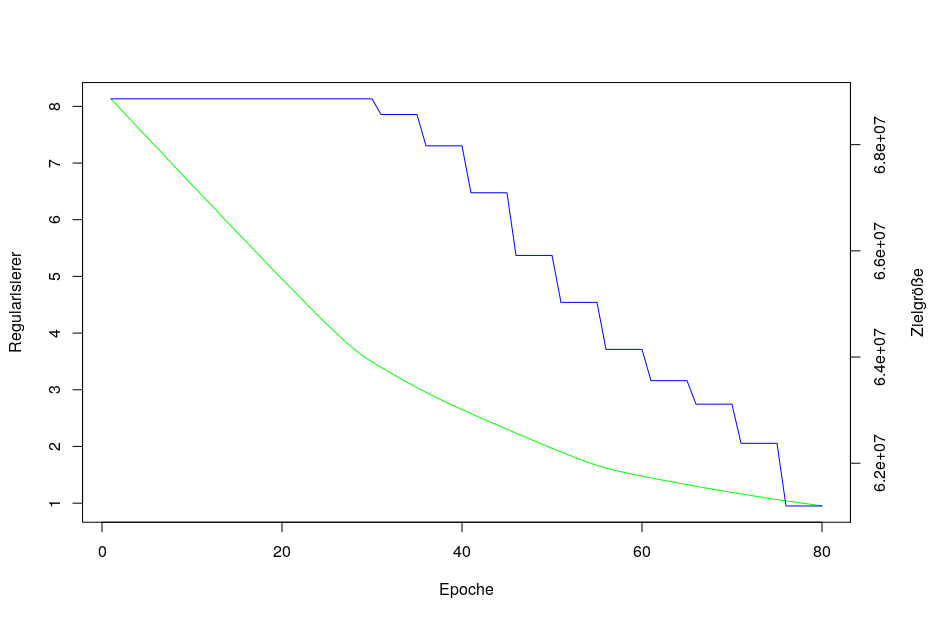
\includegraphics[width=0.47\textwidth]{KapitelPartB/Images/morph1.png}\label{abb:morphFLOPs}}
     \hfill
     \subfloat[][]{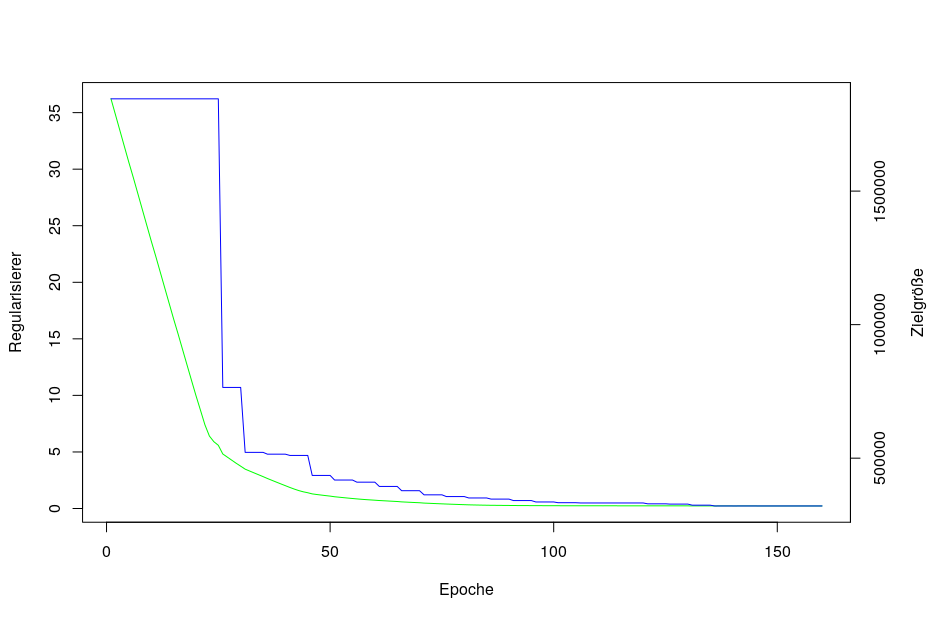
\includegraphics[width=.47\linewidth]{KapitelPartB/Images/morph2.png}\label{abb:morphSize}}
     \caption{Vergleich Zielgröße mit Wert des Regularisierers für (a) FLOPs (b) Modellgröße }
     \label{abb:morph1}
\end{figure}


Der Effekt von verschieden großen $\lambda$ wird im nächsten Schritt untersucht. Zu diesen Zweck wird ein Netzwerk mit verschiedenen Werten für $\lambda$ trainiert. Dabei wird das Netz jeweils für 180 Epochen trainiert und anschließend wird das Netz beschnitten. Abhängig von der Größe von $\lambda$ wird dem Regularisierer mehr oder weniger Gewicht gegeben. In Abbildung \ref{abb:morph3} ist zu sehen, wie sich der MorphNet Algorithmus bei verschiedenen $\lambda$ für die Zielgröße FLOPs verhält. In Abbildung \ref{abb:morph4} ist abgebildet wie sich die Netzverkleinerungsraten verändern, bei der Zielgröße Modellgröße. In der Originalveröffentlichung wurde der Effekt von verschiedenen $\lambda$ untersucht und für die Zielgröße FLOPs auch dargestellt. Dabei zeigte sich, dass mit verschiedenen Werten von $\lambda$ eine Kurve gebildet werden konnte, die für das Verhältnis zwischen Flops per Inferenz und der Accuracy einen Zusammenhang findet: Je kleiner die Flops Anzahl ist, so geringer ist auch die Accuracy \cite{morphnet}. Wie in Abbildung \ref{abb:morph3} für die Zielgröße Flops zu sehen ist, ist dieser Zusammenhang für ein ResNet nicht zu finden. Die Accuracy der hier angegebenen Netze ist im so gering, da viel vom Netz weggeschnitten wird, beziehungweise durch den Regularisierer minimiert wurden. Durch die große Verkleinerungsrate sind auch größere Veränderungen an der Struktur möglich.


In Abbildung \ref{abb:morph5} ist abgebildet, wie sich die Zielgröße Flops im Zusammenhang mit der Accuracy verändert, bei einem festen $\lambda = 3 \cdot 10^{-8}$. Im Vergleich zeigt sich jetzt das in Abbildung \ref{abb:morph4} für mehrere verschiedene $\lambda$ eine Accuracy Spanne von 6.43 \% ergibt. Bei $\lambda = 3 \cdot 10^{-8}$ ergibt sich eine Spanne von 5,72 \%. Damit zeigt sich, dass das Ergebnis nach einem Beschneidungsvorgang nicht stabil ist. Dies könnte an der generellen Instabilität des Trainings liegen (stark sich verändernde Accuracy- Werte) oder an strukturellen Unterschieden zum Inception Netz. Wie in Kapitel \ref{sec:inception} geschrieben unterscheidet sich das ResNet vom Inception Netz durch das Fehlen von Kurzschlussverbindungen, das Anwenden mehrere Filter im Inception Netz und der Tiefe vom Inception Netz. Ein weiterer Unterschied, der für das unterschiedliche Abschneiden verantwortlich sein. könnte ist die Verwendung von Cifar 10 statt Imagenet.


In Tabelle \ref{tab:time} sind die durchschnittlichen Trainingszeiten für die Zielgröße FLOPs im Vergleich mit dem Baseline-Netz zu sehen. Der Unterschied zwischen den verschiedenen Werten von $\lambda$ zeigt und dem breiten Baseline-Netz zeigt, dass etwa 3,5 Sekunden zwischen der durchschnittlichen Trainingszeit des Baseline-Netzes und den durchschnittlichen Trainingszeiten von MorphNet mit den vier verschiedenen $\lambda$. Da hier nur einmal beschnitten wird hauptsächlich gemessen, wie viel Overhead durch das Berechnen des Regularisierers entsteht.
\begin{table}[]
\begin{tabular}{c|c|c|c|c|c|}
\cline{2-6}
                                                      & Baseline & $1\cdot 10^{-8}$   & $2\cdot 10^{-8}$   & $3\cdot 10^{-8}$   & $4\cdot 10^{-8}$   \\ \hline
\multicolumn{1}{|l|}{durchschnittliche Trainingszeit} & 19,57    & 23,13 & 23,03 & 23,07 & 23,10 \\ \hline
\end{tabular}
\caption{Durchschnittliche Trainingszeiten verschiedener $\lambda$ und dem Baseline-Netz}
\label{tab:time}
\end{table}

\begin{figure}
     \centering
     \subfloat[][]{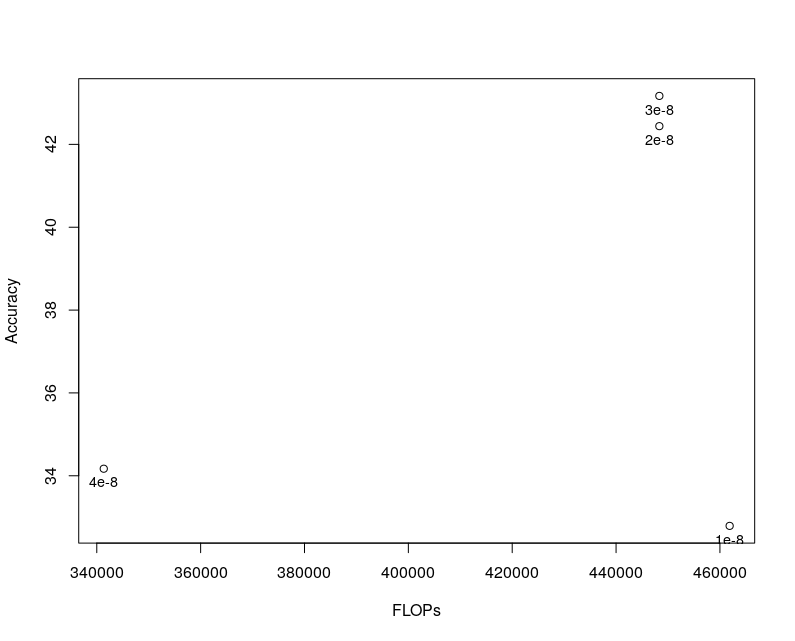
\includegraphics[width=0.47\textwidth]{KapitelPartB/Images/morph3.png}\label{abb:morph3}}
     \hfill
     \subfloat[][]{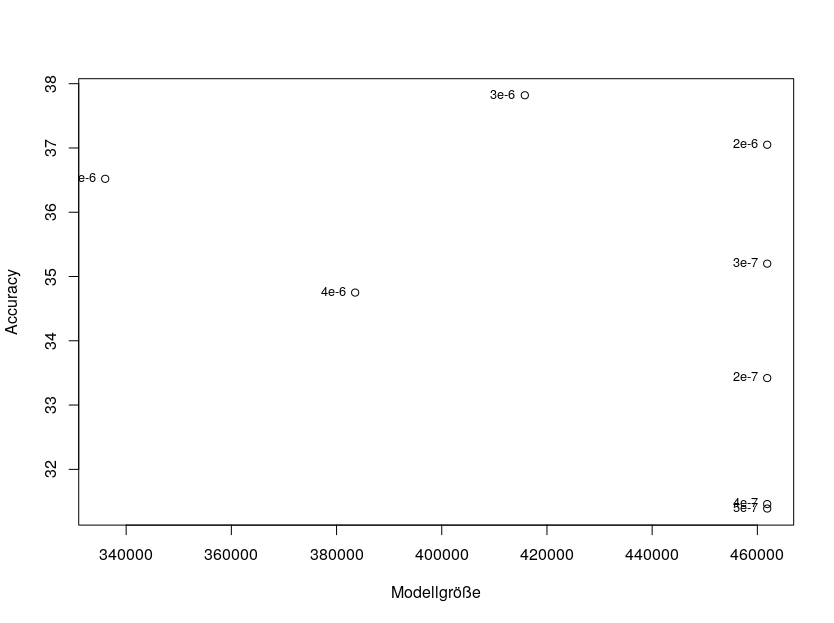
\includegraphics[width=.47\linewidth]{KapitelPartB/Images/morph4.png}\label{abb:morph4}}
     \subfloat[][]{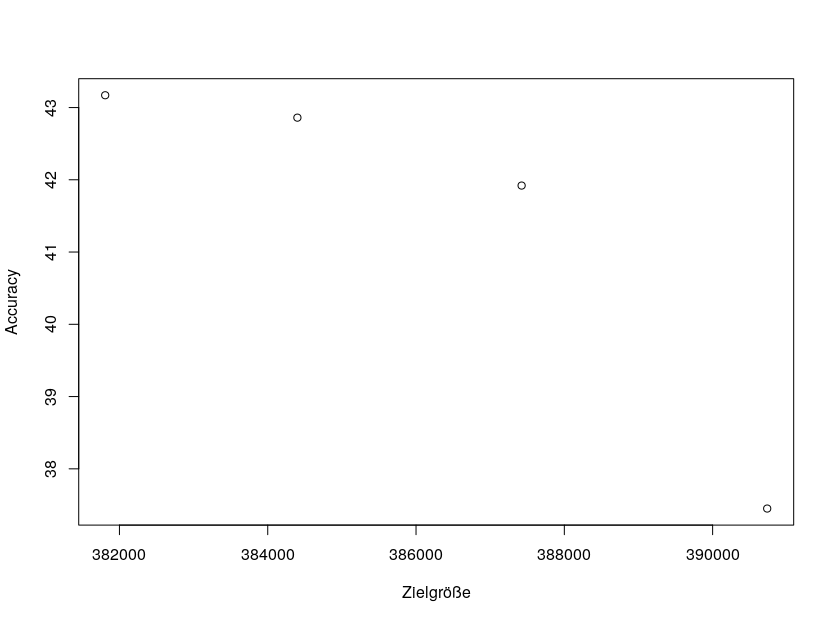
\includegraphics[width=.47\linewidth]{KapitelPartB/Images/morph5.png}\label{abb:morph5}}
     \caption{Effekt verschieden großer $\lambda$ auf  (a) FLOPs (b) Modellgröße. (c) Effekt verschiedener Experimente bei festem $\lambda$ }
     \label{abb:morph2}
\end{figure}
Da sich aus dem Experiment für die verschiedenen $\lambda$ kein Kandidat mittels einer Heuristik aussuchen lässt findet die Evaluierung in nächsten Unterkapitel mit mehreren $\lambda$ statt.


\section{Evaluierung der Ergebnisse von MorphNet}

Um zu evaluieren, wie gut MorphNet auf einem ResNet mit Cifar10 abschneidet wird der MorphNet Algorithmus für verschiedene Werte von $\lambda$ ausgeführt. Dafür wird jeweils für 30 Epochen trainiert um danach das Netz zu beschneiden. Nach dem Beschneiden wird das Netz mittels des Breitenmultiplikators auf die maximale Breite gebracht. Die maximale Breite wird durch einen erlaubten Maximalwert der Zielgröße gegeben ist. Begonnen wird mit dem schmalen Baseline-Netz. In Abbildung \ref{abb:morphAcc} ist der Verlauf der Accuracy zu sehen. Es ist zu beobachten, dass der MorphNet Algorithmus etwa das Ergebnis des breiten Baseline-Netzes erreicht. Die letzten 30 Epochen werden hier ohne den Regularisierer trainiert. 

Als Ergebnis ist zu beobachten, dass ausgehend vom schmalen Baseline-Netz mit einer durchschnittlichen Accuracy von 74 \% eine Verbesserung in den Bereich der Accuracy des breiten Baseline-Netzes gelingt.  
\begin{figure}
\begin{verbatim}
BasicBlock(
    (0): Conv2d(76, 76, kernel_size=(3, 3), stride=(2, 2),
    padding=(1, 1))
    (1): BatchNorm2d(76, eps=1e-05, momentum=0.1, affine=True,
    track_running_stats=True)
    (2): ReLU(inplace=True)
    (3): Conv2d(76, 76, kernel_size=(3, 3), stride=(1, 1), 
    padding=(1, 1))
    (4): BatchNorm2d(76, eps=1e-05, momentum=0.1, affine=True, 
    track_running_stats=True))
\end{verbatim}
\caption{Struktur eines Basisblocks als Ergebnis von MorphNet 1}
\label{abb:verb1}
\end{figure}
\begin{figure}
\begin{verbatim}   
BasicBlock(
    (0): Conv2d(76, 5, kernel_size=(3, 3), stride=(1, 1), 
    padding=(1, 1))
    (1): BatchNorm2d(5, eps=1e-05, momentum=0.1, affine=True, 
    track_running_stats=True)
    (2): ReLU(inplace=True)
    (3): Conv2d(5, 76, kernel_size=(3, 3), stride=(1, 1), 
    padding=(1, 1))
    (4): BatchNorm2d(76, eps=1e-05, momentum=0.1, affine=True, 
    track_running_stats=True))
\end{verbatim}
\caption{Struktur eines Basisblocks als Ergebnis von MorphNet 2}
\label{abb:verb2}
\end{figure}

In den Abbildungen \ref{abb:verb1} und \ref{abb:verb2} sind beispielhaft zwei Basisblöcke zu sehen, wie sie Bestandteil des Netzes nach Durchlaufen des MorphNet-Algorithmus sind. Zu beobachten ist, dass es sowohl Blöcke mit sehr wenig inneren Kanälen gibt als auch Blöcke, die viele innere Kanäle haben. Hier wäre eine Untersuchung, welchen Effekt diese Blöcke mit schmalem Inneren haben interessant.

\begin{figure}
     \centering
     \subfloat[][]{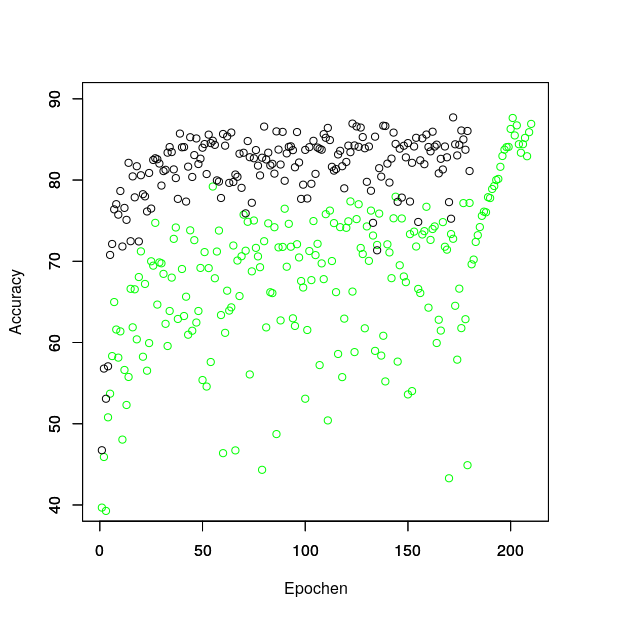
\includegraphics[width=0.47\textwidth]{KapitelPartB/Images/morph6.png}\label{abb:morph6}}
     \hfill
     \subfloat[][]{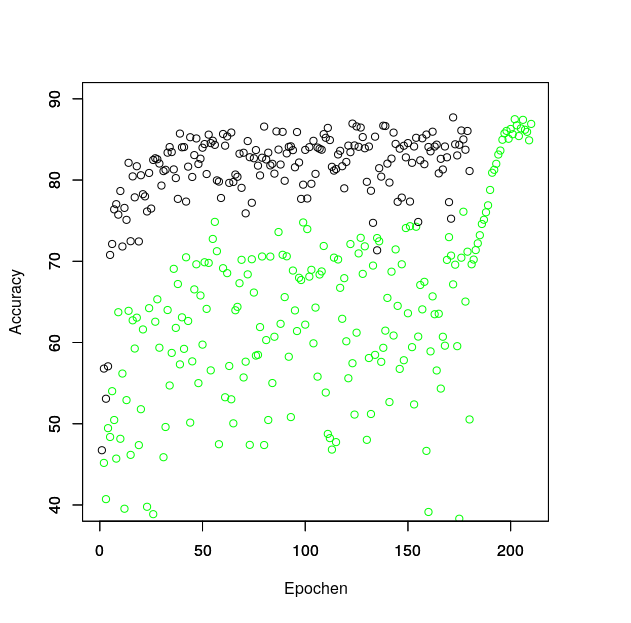
\includegraphics[width=.47\linewidth]{KapitelPartB/Images/morph7.png}\label{abb:morph7}}\\
     \subfloat[][]{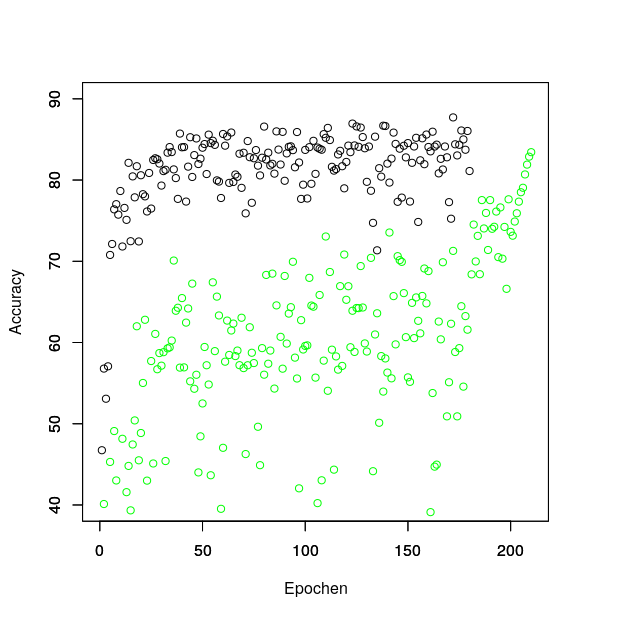
\includegraphics[width=.47\linewidth]{KapitelPartB/Images/morph8.png}\label{abb:morph8}}
     \subfloat[][]{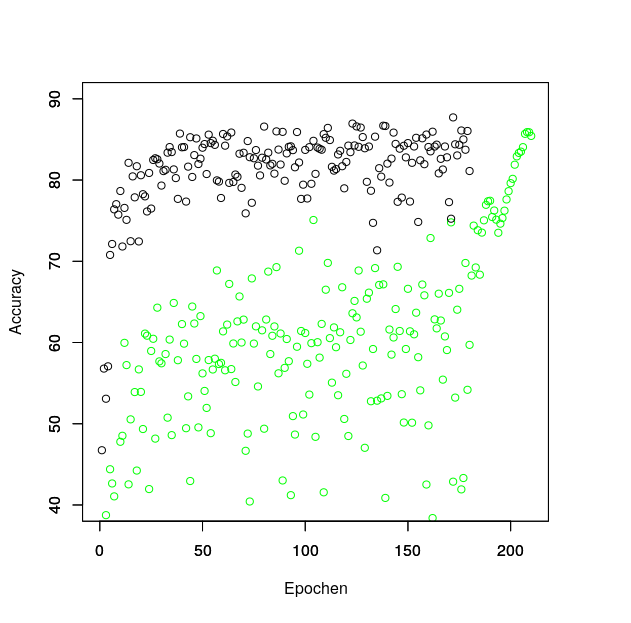
\includegraphics[width=.47\linewidth]{KapitelPartB/Images/morph9.png}\label{abb:morph9}}\\
     \subfloat[][]{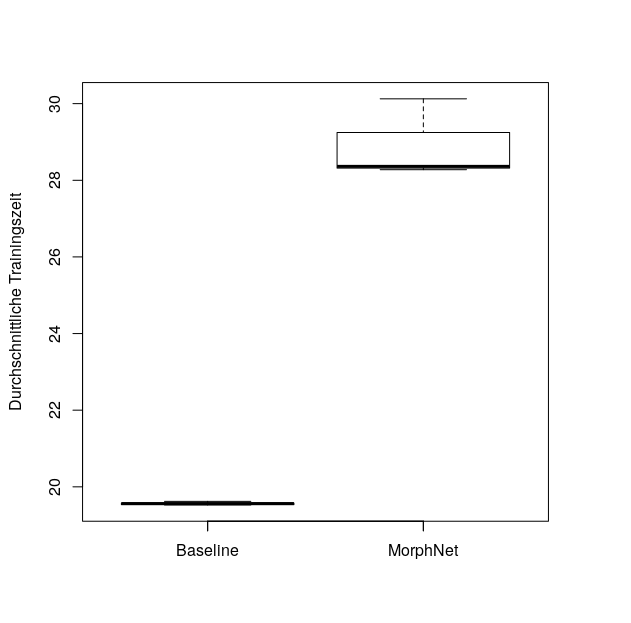
\includegraphics[width=.47\linewidth]{KapitelPartB/Images/morphTime.png}\label{abb:morphTime}}

     \caption{Effekt verschieden großer $\lambda$ auf die Accuracy nach 210 Epochen im Vergleich zum Baseline Netz für (a) $\lambda = 1 \cdot 10^{-8}$ (b) $\lambda = 2 \cdot 10^{-8}$ (c) $\lambda = 3 \cdot 10^{-8}$ (d) $\lambda = 4 \cdot 10^{-8}$. (e) Boxplot zum Vergleich der durchschnittlichen Trainingszeit von Baseline Netz mit dem MorphNet Netz}
     \label{abb:morphAcc}
\end{figure}

Im Gegensatz zur Veröffentlichung kann mit den durchgeführten Experimenten keine Struktur gefunden werden, die besser abschneidet als das Baseline Netz. Möglicherweise ist das Netz hier nach 210 Epochen noch nicht fertig trainiert.
Eine weitere Möglichkeit ist, dass ein besseres Abschneiden des ResNets mit Cifar10 nicht durch eine bessere Struktur mit der Beschränkung der Zielgröße möglich ist. Für diesen Grund spricht, dass mittels Net2Net eine bessere breitere Struktur gefunden wurde, in dem das komplette Baseline Netz mit dem Faktor zwei in der Breite verdoppelt wurde. 

In Abbildung \ref{abb:morphTime} ist zu sehen wie die hier durchgeführten Experimente zeitlich abschneiden.  
Um zu überprüfen, wie groß die Wahrscheinlichkeit für einen Fehler 1. Art ist wird zwischen den durchschnittlichen Trainingszeit des Baseline Netzes und des MorphNet Netzes ein t-Test durchgeführt. Es ergibt sich ein p-Wert von 0.0002. Damit sind die Zeiten des MorphNet Algorithmus hier signifikant höher, als beim Baseline Netz. 









\begin{comment}
\chapter{Additive Verfahren}

\subsection{Zahlenformate}\label{sec:zahlen}
\todo[inline]{Text fertig schreiben; etwa 4 Stunden}
\begin{itemize}
 \item FP16 bereits probiert
\end{itemize}


FP16 nur auf RTX 2080 sinnvoll
Bietet nach erster Messung etwa 28 \% Prozent Gewinn.

Code für dieses Verfahren liegt vor: Amp apex von Nvidia

AMP bietet 3 mögliche Optimierungsstufen:

O1
Patch all Torch functions and Tensor methods to cast their inputs according to a whitelist-blacklist model. Whitelist ops (for example, Tensor Core-friendly ops like GEMMs and convolutions) are performed in FP16. Blacklist ops that benefit from FP32 precision (for example, softmax) are performed in FP32. O1 also uses dynamic loss scaling, unless overridden.

02
casts the model weights to FP16, patches the models forward method to cast input data to FP16, keeps batchnorms in FP32, maintains FP32 master weights, updates the optimizer’s paramgroups so that the optimizer.step() acts directly on the FP32 weights (followed by FP32 master weight-FP16 model weight copies if necessary), and implements dynamic loss scaling (unless overridden). Unlike O1, O2 does not patch Torch functions or Tensor methods.


O3
may not achieve the stability of the true mixed precision options O1 and O2. However, it can be useful to establish a speed baseline for your model, against which the performance of O1 and O2 can be compared. If your model uses batch normalization, to establish speed of light you can try O3 with the additional property override keepBatchnormfp32=True (which enables cudnn batchnorm, as stated earlier).

Hier nur O0, O1 und O2 dargestellt, da O3 absolut nicht mithalten kann was Performance angeht.

\begin{figure}[h]
 \centering
 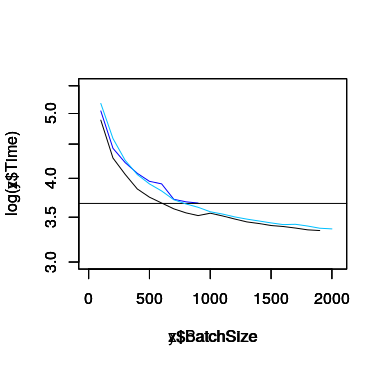
\includegraphics[width=0.8\textwidth]{KapitelPartB/Images/timeVsBatchSize_Amp.png}
 % timeVsBatchSize_Amp.png: 387x367 px, 96dpi, 10.24x9.71 cm, bb=0 0 290 275
 \caption{Vergleich Trainingszeit einer Epoche für verschiedene Optimierungsstufen von Amp Apex. DunkelBlau=O0; Schwarz = O1; Hellblau=O2}
 \label{fig:amp}
\end{figure}
\url{https://developer.download.nvidia.com/video/gputechconf/gtc/2019/presentation/s9998-automatic-mixed-precision-in-pytorch.pdf} zeigt, dass bezüglich der Accuracy kein Verlust zu erwarten ist.

Da O2 gegenüber O1 keinen signifikanten zusätzlichen Gewinn bringt nutze O1.



\subsection{LARS}\label{sec:lars}
\todo[inline]{Experimente fast fertig (3x mal auf einer Graka für 50 min); dann etwa 3 Stunden fürText + Evaluierung}




Es stellt sich die Frage, ob das einen so grossen Einfluss auf die Ausführungszeit hat.



Man sieht, dass mit steigender Batchgröße die Ausführungszeit sinkt. 

Errechne zusätzlich noch ein Modell, wo abhängig von der Modellgrösse währenddem Pruning die Batchgrösse angepasst wird.





\subsection{Beschleunigung der Berechnung des Gradientenabstiegverfahren}
\todo[inline]{ab hier löschen}

Accelerating CNN Training by Sparsifying Activation Gradients funktioniert nur auf Toy-Benchmarks 


\subsubsection{Weight Normalization: A Simple Reparameterization
to Accelerate Training of Deep Neural Networks}


Könnte funktionieren. Code für Lasagne: https://github.com/TimSalimans/weight\_norm


\subsubsection{Accelerating Deep Neural Network Training with Inconsistent Stochastic Gradient Descent}

Interessant bisher kein Code verfügbar

\subsubsection{Accelerated CNN Training Through Gradient Approximation }

Interessant bisher kein Code verfügbar


\end{comment}
